\documentclass[11pt]{article}
\usepackage{pifont}
\usepackage{multicol}
\usepackage{listings}
\usepackage{pgf}
\usepackage{tikz}
\usepackage{alltt}
\usepackage{hyperref}
\usepackage{url}
\usepackage{amssymb}
\usetikzlibrary{arrows,automata,shapes,positioning}
\tikzstyle{block} = [rectangle, draw, fill=blue!20, 
    text width=5em, text centered, rounded corners, minimum height=2em]
\tikzstyle{bt} = [rectangle, draw, fill=blue!20, 
    text width=1em, text centered, rounded corners, minimum height=2em]
\newcommand{\xmark}{\ding{55}}

\newtheorem{defn}{Definition}
\newtheorem{crit}{Criterion}
\newcommand{\true}{\mbox{\sf true}}
\newcommand{\false}{\mbox{\sf false}}

\newcommand*\circled[1]{\tikz[baseline=(char.base)]{
            \node[shape=circle,draw,inner sep=2pt] (char) {#1};}}


\newcommand{\handout}[5]{
  \noindent
  \begin{center}
  \framebox{
    \vbox{
      \hbox to 5.78in { {\bf Software Testing, Quality Assurance and Maintenance } \hfill #2 }
      \vspace{4mm}
      \hbox to 5.78in { {\Large \hfill #5  \hfill} }
      \vspace{2mm}
      \hbox to 5.78in { {\em #3 \hfill #4} }
    }
  }
  \end{center}
  \vspace*{4mm}
}

\newcommand{\lecture}[4]{\handout{#1}{#2}{#3}{#4}{Lecture #1}}
\topmargin 0pt
\advance \topmargin by -\headheight
\advance \topmargin by -\headsep
\textheight 8.9in
\oddsidemargin 0pt
\evensidemargin \oddsidemargin
\marginparwidth 0.5in
\textwidth 6.5in

\parindent 0in
\parskip 1.5ex
%\renewcommand{\baselinestretch}{1.25}

\usepackage{enumitem}

\newtheorem{prop}{Proposition}
\newtheorem{lemma}{Lemma}
\usepackage{ebproof}
\newcommand{\qedsymbol}{\rule{1ex}{1ex}}
\newcommand{\sem}[3]{\langle #1, #2 \rangle \Downarrow #3}

\lstset{ %
language=Java,
basicstyle=\ttfamily,commentstyle=\scriptsize\itshape,showstringspaces=false,breaklines=true,numbers=left}

%\usepackage{fontspec}
%\setmonofont{Cousine}[Scale=MatchLowercase]

\begin{document}

\lecture{12 --- February 26, 2025}{Winter 2025}{Patrick Lam}{version 1}

We've seen this picture on the slides.

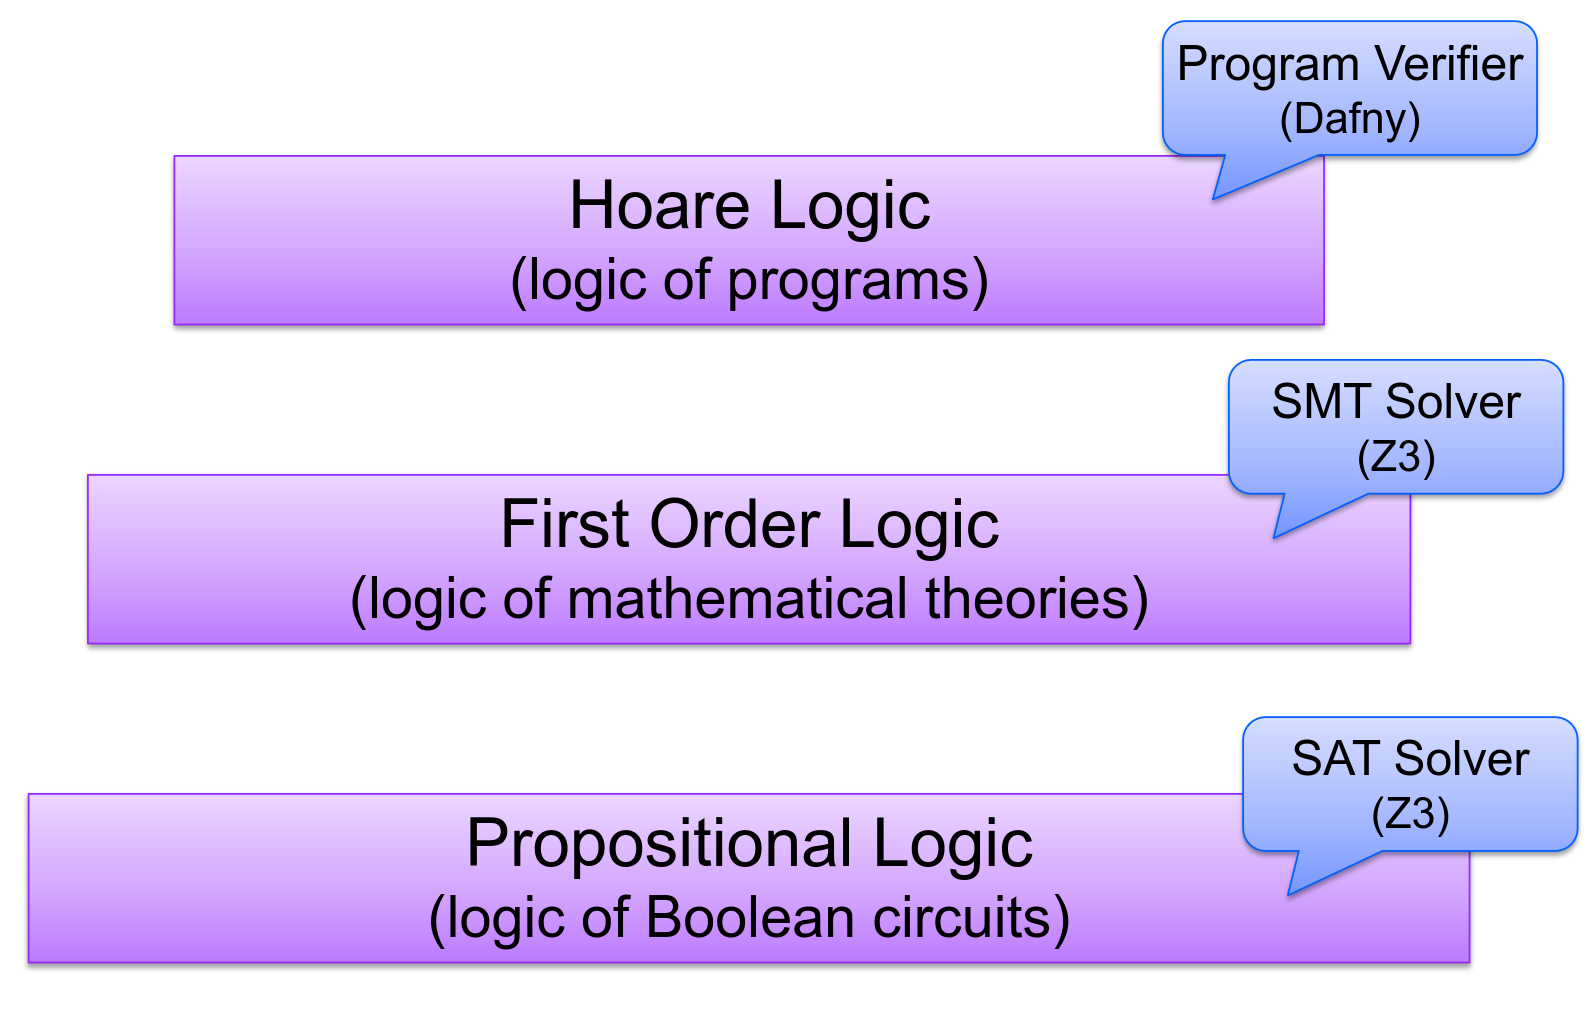
\includegraphics[width=\textwidth]{L12/three-logics.png}

This lecture is about Hoare Logic. Again, you've seen this in SE 212, but it's worth a review as we
prepare to move onto Dafny. Some of the concepts are subtle!

%https://www.site.uottawa.ca/~afelty/csi5137/plf/Hoare.html
%https://cs.stackexchange.com/questions/118322/why-is-the-assignment-rule-the-way-it-is-in-hoare-logic
%https://www.cs.cornell.edu/courses/cs4160/2019sp/terse/plf/Hoare.html

\paragraph{Axiomatic Semantics.} You used axiomatic semantics in SE 212.
It consists of:
\begin{itemize}[noitemsep]
\item a language for stating assertions about programs; and
  \item rules for establishing the truth of assertions.
\end{itemize}

You have used axiomatic semantics to make and prove assertions. Some examples:
\begin{itemize}[noitemsep]
\item this program terminates;
\item if this program terminates, the variables \texttt{x} and \texttt{y} have the same value throughout the execution of the program;
\item array accesses are within array bounds.
\end{itemize}

One can use first-order logic for assertions. There are also
special-purpose specification languages, which I'll name-check but not
discuss: Z (the OG specification language), Larch, JML.  And there are
other logics as well: temporal logic, especially useful for specifying
properties of concurrent systems; linear logic, which has been used
under-the-hood for Rust uniqueness; and separation logic, for
reasoning about the structure of the heap.

\paragraph{Hoare Triples.} We write assertions about WHILE programs using Hoare triples:
\[ \{ A \} ~c~ \{ B \} \]
which means that (1) if $A$ holds in state $q$, and (2) if the semantics says $q \rightarrow q'$, then (3) $B$ holds in $q'$.

One can thus write the valid assertion
\[ \{ y \leq x \} z := x; z := z + 1 \{ y < z \} \]
which means that if $y \leq x$ and you run those two statements, you know that $y < z$ at the end of them.

\paragraph{Partial versus total correctness.} More specifically, $\{A\} ~c~ \{ B\}$ is a \emph{partial} correctness assertion,
and does not imply termination of $c$.

If $A$ holds in state $q$, and if there exists $q'$ such that $q \rightarrow q'$, then $B$ holds in state $q'$. So,
if there is no $q'$ (i.e. $c$ does not terminate, or gets stuck), then there is, vacuously, no obligation to show $B$.

There is the notion of \emph{total} correctness as well, though much less often used. $[A] ~c~ [B]$ is the notation for
\emph{total} correctness.

If $A$ holds in state $q$, {\bf then} there exists $q'$ such that $q \rightarrow q'$, and $B$ holds in state $q'$.

\subsection*{More formal Hoare logic}
We have assertions like $A$ and $B$. We'll formalize the language we use for them,
define when an assertion holds in a state, and define rules for deriving valid Hoare triples.

\paragraph{Our assertion language.}
We use \emph{first-order predicate logic} and use WHILE expressions as atoms.

\begin{eqnarray*}
  A &::==& \mathsf{true} \mid \mathsf{false} \mid e_1 = e_2 \mid e_1 \geq e_2 \\
  &\mid& A_1 \wedge A_2 \mid A_1 \vee A_2 \mid A_1 \Rightarrow A_2 \mid \forall x. A \mid \exists x. A
\end{eqnarray*}
There are logical variables (e.g. $\forall x$) and program variables.
We don't distinguish them. For our purpose, all WHILE variables range over integers.

It is always valid to use a WHILE Boolean expression as an assertion.

\paragraph{Semantics of assertions.}
We write
\[ q \models A \]
to mean that assertion $A$ holds in state $q$.
(It is well-defined when $q$ is defined on all variables occuring free in $A$).

We define $\models$ inductively on the structure of assertions. (Start with the atomic assertions
and arithmetic expressions from WHILE, and then build up the compound assertions like $\wedge$ etc.)

\[
\begin{array}{ll}
  q \models \mathsf{true} & \mbox{always} \\
  q \models e_1 = e_2 &    \mbox{iff~} \sem{e_1}{q}{}~ = \sem{e_2}{q}{} \\
  q \models e_1 \geq e_2 & \mbox{iff~} \sem{e_1}{q}{}~ \geq \sem{e_2}{q}{} \\
  q \models A_1 \wedge A_2 & \mbox{iff~} q \models A_1 \mathrm{~and~} q \models A_2 \\
  q \models A_1 \vee A_2 & \mbox{iff~} q \models A_1 \mathrm{~or~} q \models A_2 \\
  q \models A_1 \Rightarrow A_2 & \mbox{iff~} q \models A_1 \mathrm{~implies~} q \models A_2 \\
  q \models \forall x.~ A & \mbox{iff~} \forall n \in \mathbb{Z}.~q[x:=n] \models A\\
  q \models \exists x.~ A & \mbox{iff~} \exists n \in \mathbb{Z}.~q[x:=n] \models A\\
\end{array}
\]
  
\end{document}
